\label{cap:standDerTechnik}
Dieses Kapitel befasst sich mit dem aktuellen Stand der Technik. Dies
umfasst sowohl die gegenw{\"a}rtig eingesetzte Hardware (Rover Curiosity, Deep
Space Antennen), als auch bereits entwickelte Protokolle zur interplanetaren
Kommunikation (Bundle-Protokoll etc.). Abschlie{\ss}end wird ein Bezug zum im
Zuge dieser Arbeit implementierten Relevance-Oriented Transport Protocol
hergestellt. Zudem wird eine Einordnung der vorgestellten Protokolle in
den Stack einer interplanetaren Kommunikation vorgenommen. Au{\ss}erdem wird ein
Vergleich der Handhabung von relevanten Daten innerhalb der unterschiedlichen
Protokolle aufgezeigt. Im Zuge dessen wird Bezug auf die im \gls{CRODT}-Framework
eingesetzte \gls{CROP} genommen \cite{Daher}.

\section{Weltraum-Technologien}

\textbf{Mars Rover Curiosity} \newline

Der Mars Rover \textit{Curiosity} (Abbildung \ref{fig:Curiosity}) verf{\"u}gt
{\"u}ber einen RAD750 Prozessor von BAE-Systems.
Dieser hat eine Taktfrequenz von bis zu 200 MHz und kann 266 MIPS
verarbeiten\footnote{Dieser Prozessor ist verglichem mit der Hardware, die im
Verlauf dieser Arbeit zum Test des entwickelten Protokolls eingesetzt wurde
sehr schwach.}. Desweiteren verf{\"u}gt \textit{Curiosity} {\"u}ber einen
Arbeitsspeicher von 256 MB und einen Flash-Speicher von 2 GB. Zus{\"a}tzlich
hat \textit{Curiosity} einen EPROM von 256 KB. Alle Bauteile sind dabei
besonders strahlungsresistent und unempfindlich gegen{\"u}ber gro{\ss}en
Temperaturschwankungen. Das genutzte Betriebssystem ist VxWorks \cite{WR}.
Zur Kommunikation nutzt der Rover einerseits das X-Band (7 - 8 GHz), welches zur
{\"U}bertragung von Statusdaten und zum Empfang von Steuerdaten genutzt wird.
Des Weiteren verf{\"u}gt der Rover {\"u}ber ein Kommunikationssystem im UHF-Band
(0,4 GHz), welches f{\"u}r wissenschaftliche Daten mit hohem Datenvolumen
genutzt wird (bis zu 250 Mbit pro Tag, somit ca. 30 MB/Tag).\newline 
Die Ausstattung an wissenschaftlichen Instrumenten umfasst zehn Ger{\"a}te.
Darunter z.B. zwei Mastkameras welche je eine Aufl{\"o}sung von 1.200 x 1.200
Pixeln haben (1,44 Megapixel). Diese Kameras sind ebenfalls in der Lage
720p-Videos mit einer Framerate von 10 Bildern pro Sekunde aufzunehmen. Hinzu
kommen Spektrografen, weitere Kameras, Sensoren etc., welche weitere
Analysedaten beisteuern \cite{web5}. Anhand der Vielzahl von Messinstrumenten,
Kameras etc. wird erkennbar, dass eine Menge unterschiedlicher Datentypen zu
verwalten ist.
Desweiteren zeigt beispielsweise die Aufl{\"o}sung der Mastkameras, dass zudem
auch gro{\ss}e Datenmengen zu verwalten sind. Diese Anforderungen gilt es in den
verwendeten Kommunikationsprotokollen zu ber{\"u}cksichtigen.

\begin{figure}[H]
	\centering
	\includegraphics[scale=.14]{Curiosity.png}
	\caption[Mars Rover Curiosity]{Mars Rover Curiosity \cite{imgCuriosity}}
	\label{fig:Curiosity}
\end{figure}

\textbf{Deep Space Network} \newline

Das Deep Space Network bezeichnet ein Netz von Parabolantennen, welche zur
Kommunikation mit Raumsonden, Satelliten sowie zu radio-
und radarastronomischen Zwecken dienen. F{\"u}r die NASA werden derzeit die
folgenden drei gro{\ss}en Stationen betrieben:

\begin{compactenum}[a)]
	\item \textit{Goldstone Deep Space Communication Complex, Kalifornien, USA
	(Abbildung} \ref{fig:Goldstone}\textit{)}
	\item \textit{Madrid Deep Space Communication Complex, Madrid, Spanien}
	\item \textit{Canberra Deep Space Communication Complex, Canberra, Australien}
\end{compactenum}

Das Deep Space Network wird auch f{\"u}r die Kommunikation zwischen dem Mars
Rover \textit{Curiosity} und der Erde genutzt. Die Anlagen liegen an exponierter Position
(zumeist h{\"u}geliges schalenf{\"o}rmiges Gel{\"a}nde). Dies soll den
Einfluss von St{\"o}rungen z.B. durch Radiofrequenzen reduzieren. Die Stationen
befinden sich je in einem Abstand von einem drittel Erd{\"a}quator, um eine
fortw{\"a}hrende Kommunikation mit Raumfahrzeugen trotz Erdrotation zu
erm{\"o}glichen \cite{web6}.

\begin{figure}[H]
	\centering
	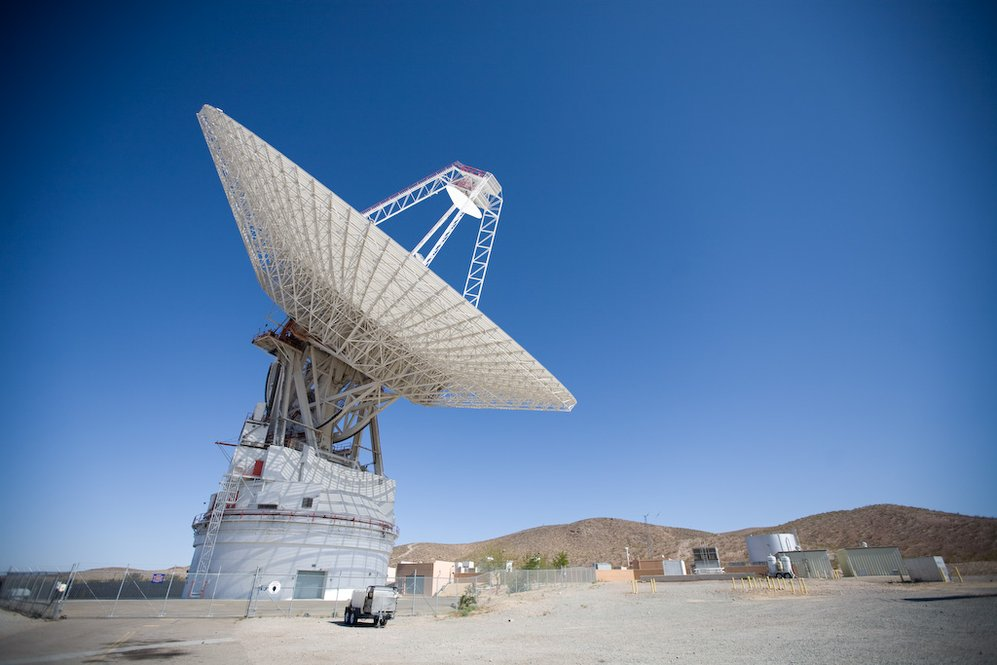
\includegraphics[scale=.3]{Goldstone.jpg}
	\caption[Antenne der NASA Deep Space Network Einrichtung in Goldstone, Kalifornien, USA]
	{Antenne der NASA Deep Space Network Einrichtung in Goldstone, Kalifornien, USA \cite{imgGoldstone}}
	\label{fig:Goldstone}
\end{figure}

\section{Definitionen}

\textbf{Interplanetary Internet}

Das \gls{IPN} bezeichnet die Erweiterung des Internets
auf einen au{\ss}erirdischen Bereich. Die damit verbundenen {\"A}nderungen im
Vergleich zum irdischen Internet umfassen z.B. einen gesonderten Umgang mit
Latenzen, da diese beim \gls{IPN} im Minuten- bis Stundenbereich liegen. Die
Entwicklung von Protokollen f{\"u}r das \gls{IPN} obliegt dabei dem \gls{CCSDS}.

\textbf{Delay Tolerant Networking}

Das \gls{DTN} bezeichnet eine Protokollarchitektur f{\"u}r
Ende-zu-Ende Netzwerkverbindungen mit geringer Stabilit{\"a}t. Die Basis der
\gls{DTN} Netzwerkarchitektur stellt das von der NASA entwickelte \gls{IPN} dar. Ein wichtiger
Bestandteil dieser Netzwerke ist der Umgang mit gro{\ss}en Latenzen. Zudem
m{\"u}ssen die an der Kommunikation beteiligten Knoten (Teilnehmer)
Daten solange zwischenspeichern, bis der Empf{\"a}nger den Erhalt quittiert hat
(store-and-forward) \cite{web3}.

\section{Protokolle}

\textbf{Bundle-Protokoll}

Die in den RFCs 4838 und 5050 festgelegten Anforderungen f{\"u}r \gls{DTN} sind
weitgehend unter der Bezeichnung Bundle-Protokoll bekannt. In diesem werden
Folgen von Datenbl{\"o}cken als B{\"u}ndel zusammengefasst. Jedes B{\"u}ndel enth{\"a}lt
dabei ausreichende semantische Informationen, um eine etwaige Applikation
fortzusetzen. Exemplarisch sei hier ein Webbrowser angef{\"u}hrt, welcher ein
Bundle-Paket erh{\"a}lt und dadurch eine komplette Webseite anzeigt.
Die {\"U}bertragung erfolgt dabei per \textit{store-and-forward}. Neben
IP-basierenden Protokollen k{\"o}nnen auch andere Protokolle zum Einsatz kommen
(z.B. \gls{LTP}). Das Bundle-Protokoll z{\"a}hlt zu den Overlay-Netzwerken, welche
auf einer bereits bestehenden Netzwerkstruktur aufsetzen \cite{web1}.

\textbf{Licklider Transmission Protocol}

Das \gls{LTP} kann direkt auf dem Data Link Layer
aufsetzen oder aber auch unter \gls{UDP} laufen (siehe Abb. \ref{fig:LTP}). Das \gls{LTP}
wird zudem als Standard \textit{convergence layer protocol} (Zusammenfassung von
Transport- und Network-Layer) f{\"u}r das Bundle Protokoll genutzt. Das \gls{LTP}
wurde zur sicheren {\"U}bertragung von Daten zwischen einem Sender und einem
Empf{\"a}nger (Punkt-zu-Punkt) unter \gls{DTN} Bedingungen entwickelt. Das \gls{LTP}
entscheidet dabei zwischen wichtigen (red data) und unwichtigen Daten (green
data) und gew{\"a}hrleistet somit eine effiziente {\"U}bermittlung. Eine
{\"U}bertragung beginnt, sobald ein Link zwischen Sender und Empf{\"a}nger
besteht. Die zu sendenden Datenbl{\"o}cke werden beim \gls{LTP} in Segmente geteilt.
Handelt es sich um wichtige Daten, werden w{\"a}hrend des Sendevorgangs
innerhalb der im \gls{LTP} verwendeten Segmente spezielle Flags gesetzt.
Diese einfach als Checkpoints bezeichneten Signale erfordern eine Quittierung
durch den Empf{\"a}nger, um so bei einem eventuellen Verbindungsabbruch ein
erneutes Senden des jeweiligen Datenpakets auszul{\"o}sen (vergleichbar mit
\gls{TCP}). Die Daten werden solange beim Sender im Speicher (Arbeits- oder lokaler
Festspeicher z.B. Flash) vorgehalten, bis der zugeh{\"o}rige Checkpoint
quittiert wurde. Wenn ein Checkpoint nicht quittiert wird, kann durch einen
ablaufenden Timer auf der Seite des Senders ein erneutes Senden durchgeführt
werden. Sowohl das Senden als auch Empfangen eines Blocks kann per Signal
abgebrochen werden. Zudem ist die Gr{\"o}{\ss}e der Segmente einstellbar, um
diese an den jeweiligen Zweck anzupassen. Handelt es sich bei den zu sendenden
Daten um Daten mit geringerer Relevanz, so ist keine Best{\"a}tigung durch den
Empf{\"a}nger notwendig (vergleichbar mit \gls{UDP}).
Diese Daten werden direkt nach dem Versenden gel{\"o}scht \cite{web4}.

\begin{figure}[H]
	\centering
	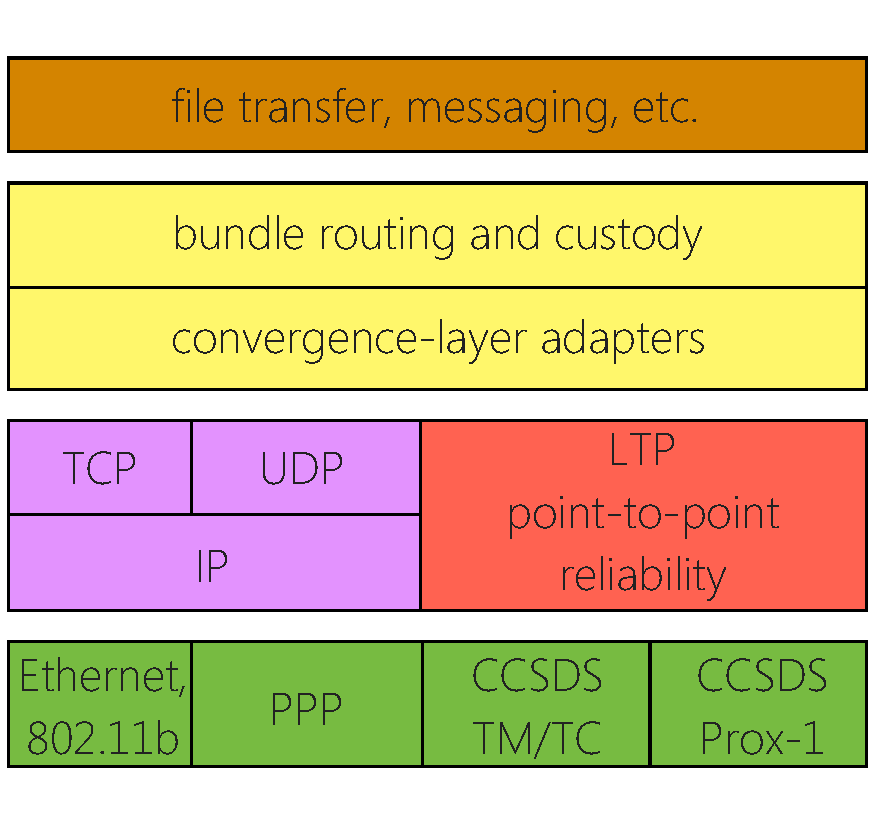
\includegraphics[scale=.4]{LTP.pdf}
	\caption[Einordnung des LTP in das Kommunikationsmodell]{Einordnung des LTP in
	das Kommunikationsmodell nach \cite{Burleigh}}
	\label{fig:LTP}
\end{figure}

\textbf{Proximity-1}

Das \textit{Proximity-1 Space Link Protocol} ist das typischerweise genutzte
Data Link Layer/Physical Layer Protokoll in einem \gls{DTN} Stack. Damit komplettiert
dies zusammen mit dem Bundle Protokoll und dem \gls{LTP} die notwendigen
Protokollschichten eines \gls{DTN} Stack in einer interplanetaren Kommunikation.

\textbf{Stack einer interplanetaren Kommunikation}

Das \gls{DTN} Bundle Protokoll agiert als ein Overlay auf dem Transport Layer. Die
Abbildung \ref{fig:PSSBN} zeigt den Einsatz des Bundle Protokolls in einem
interplanetaren Kommunikationsansatz.
Dabei repr{\"a}sentiert der linke Teil des Stacks das Landefahrzeug auf der
Marsoberfl{\"a}che, welches das \gls{CFDP} {\"u}ber das Bundle Protokoll in
Verbindung mit dem \gls{LTP} nutzt.
Das Landefahrzeug wird schlie{\ss}lich {\"u}ber das Proximity-1 Space Link
Protokoll mit dem Orbiter (zweiter Stack von links) verbunden. Der dritte Stack
von links repr{\"a}sentiert z.B. eine \gls{DSN} Bodenstation. Der
Orbiter kommuniziert mit der \gls{DSN} Bodenstation {\"u}ber einen
\textit{deep-space-link} via Bundle Protokoll unter Nutzung des \gls{LTP}. Das
\gls{LTP} gew{\"a}hrleistet dabei eine verl{\"a}ssliche Verbindung. Der Stack
auf der rechten {\"a}u{\ss}eren Seite symbolisiert eine Missionskontrollstation,
welche mit der \gls{DSN} Bodenstation {\"u}ber einen klassische
\gls{TCP}/\gls{IP} Stack kommuniziert. Das Bundle Protokoll sichert dabei eine
Ende-zu-Ende Kommunikation \cite{DTNBundle}.

\begin{figure}[H]
	\centering
	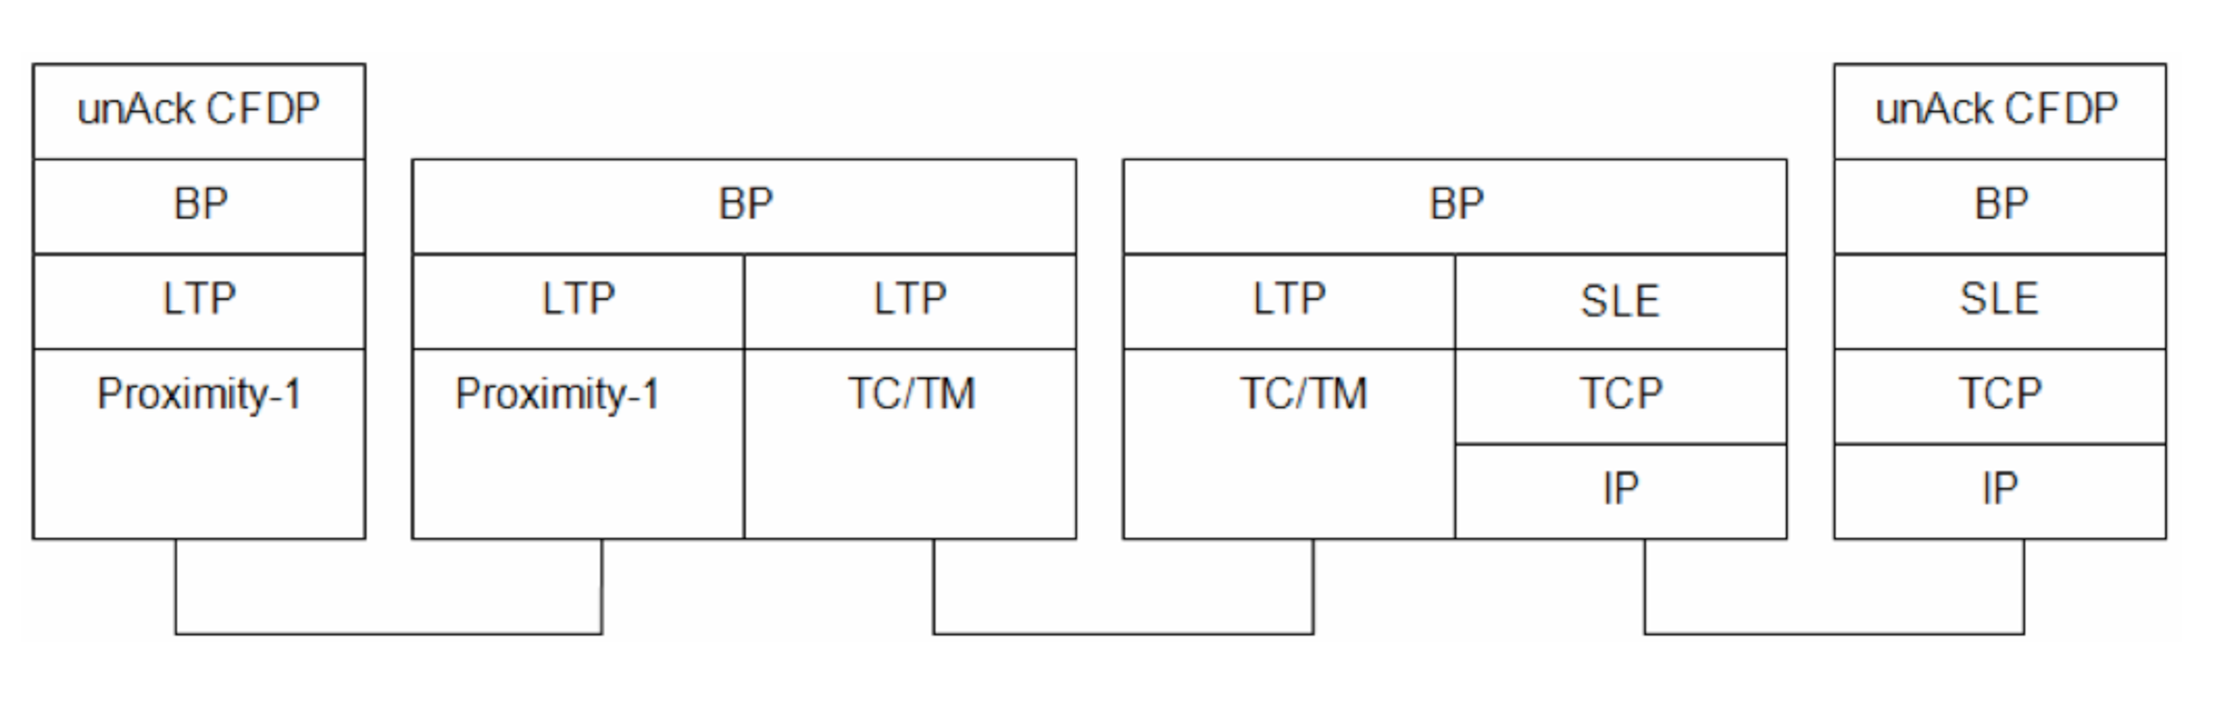
\includegraphics[width=\textwidth]{PSSBN.pdf}
	\caption[Protokoll-Stack eines interplanetaren Netzwerks]
	{Protokoll-Stack eines interplanetaren Netzwerks \cite{DTNBundle}}
	\label{fig:PSSBN}
\end{figure}

\section{Dienstg{\"u}te und Datenanalyse}

\textbf{Quality of Service}

Die G{\"u}te eines Kommunikationsdienstes wird in irdischen Netzwerken
{\"u}blicherweise als \gls{QoS} bezeichnet. Hierbei gibt es eine
Auswahl von Qualit{\"a}tsmerkmalen, mit Hilfe derer die Qualit{\"a}t eines
Service bewertet werden kann. Im Beispiel eines IP-Netzwerks w{\"a}ren dies
Parameter wie Jitter \footnote{zeitl. Fluktuation (Taktzittern) in der
{\"U}bertragung von Digitalsignalen}, Latenzzeit, die Paketverlustrate sowie der
Datendurchsatz. Mit Hilfe der gewonnenen Erkenntnisse, kann dann die
Kommunikation beeinflusst werden. Dadurch k{\"o}nnen Dienste wie z.B. ein
Video-/Audiostream ihre Ressourcennutzung verlagern bzw. anpassen
(Beispiel: Videochat sendet infolge einer Bandbreitenverschlechterung ein
st{\"a}rker komprimiertes Bild). 

\textbf{Qualitiy of Interaction} 

Das \gls{QoS}-Modell ist zwar theoretisch auch auf eine interplanetare Kommunikation
anwendbar (z.B. \gls{DTN}/\gls{IPN}), jedoch gleicht dieses aufgrund der hohen
Latenzzeiten in der {\"U}bertragung eher einer postalischen Kommunikation (\gls{QoS} hingegen
ist auf eine synchrone Kommunikation optimiert). Aus diesem Grund wurde mit dem
\gls{QoI} ein speziell f{\"u}r den asynchronen
Kommunikationsfall konzipiertes Verfahren entwickelt \cite{Daher2} (\gls{QoI}
kann auch irdische Kommunikationen verbessern). Dabei wurde ein Konzept erdacht,
welches auf Signalen basiert (Request-Signal (REQ), Response-Signal
(RSP), Information-Signal (INFO)). Mit diesen Signalen kann nun eine
Interaktion ausgel{\"o}{\ss}t werden. Die Bewertung der \gls{QoI} erfolgt in zwei Ebenen. Ebene $1$ ist die low-level \gls{QoI}. Diese befasst sich neben klassischen \gls{QoS}-Merkmalen mit der Analyse der Ausnutzung von
Kommunikationsressourcen. Die zweite Ebene wird als high-level \gls{QoI}
bezeichnet und bewertet den Erfolg einer Kommunikation.

Zur Evaluierung der low-level \gls{QoI} werden neben klassischen \gls{QoS}-Merkmalen
spezielle Merkmale zur Kommunikationsbewertung eingesetzt. Klassische
\gls{QoS}-Merkmale wie Bandbreite und Jitter k{\"o}nnen mit Hilfe der
\textit{Contact Duration} (CD), \textit{Contact Period} (CP) und des \textit{One
Way Delay} auf einen \gls{QoI}-Fall übertragen werden. Steigt z.B. die CD und
sinkt zugleich die CP so resultiert daraus eine steigende Bandbreite. Um die
Ausnutzung verf{\"u}gbarer Kommunikationsressourcen zu analysieren stehen eine
Vielzahl an Session\footnote{Kommunikationsphase, welche durch einen REQ von Sender A an
Empf{\"a}nger B gestartet wird und erst nach einem empfangenen RSP beendet
wird.}-Analysemethoden zur Verf{\"u}gung. Diese umfassen z.B. den
\textit{Session Load} (SL), die \textit{Session Duration} (SD), die
\textit{Session Signaling Rate} (SSR) oder die \textit{Sesssion Data Exchange Rate} (SDXR). Ist
z.B. die SSR gering, so ist die low-level \gls{QoI} hoch.

Das in dieser Arbeit implementierte Anwendungsszenario einer Kommunikation
zwischen Erde und Mars via \gls{CRODT}-Framework unter Nutzung einer
Chat-Applikation ist ein idealer Ansatzpunkt um die high-level \gls{QoI} zu
definieren. Diese nutzt die Ergebnisse der low-level \gls{QoI} kombiniert mit
einigen sprachspezifischen Erweiterungen \cite{Donick}. Prim{\"a}r wird dabei
{\"u}ber die SD und die SDXR in Kombination mit der \textit{Session
Coherence}\footnote{Ma{\ss} f{\"u}r den Grad an iniziierten relevanten
Anschlusshandlungen zwischen zwei Kommunikationspartnern \cite{Donick}} (SC) die
high-level \gls{QoI} evaluiert. Sind die SD und die SDXR gering und ist die SC hoch,
so ist die high-level \gls{QoI} hoch.
Der Interaktionserfolg ist daher mit hoch zu bewerten.

\textbf{Ontologien}

Ontologien sind Sammlungen aus Inferenz- und Integrit{\"a}tsregeln, um
Schlussfolgerungen auf komplexe Probleme zu beziehen. Ontologien werden zum
Austausch von Wissen in digitaler Form genutzt. Die wichtigste Bedingung einer
Ontologie ist die Allgemeing{\"u}ltigkeit. Dies unterscheidet die Ontologien von
anderen Datenmodellen, welche speziell an einen bestimmten Zweck angepasst
werden.
Bestandteile einer Ontologie:

 \begin{compactenum}[I]
   \item \textit{Begriffe}
   \item \textit{Typen}
   \item \textit{Instanzen}
   \item \textit{Relationen}
   \item \textit{Vererbung}
   \item \textit{Axiome}
 \end{compactenum}
   
 \textbf{Begriffe} werden auch als Klassen bezeichnet. Diese
 k{\"o}nnen in einer Klassenstruktur mit {\"U}ber- und Unterklasse angeordnet
 werden. Sie stellen Sammlungen von Objekten gleicher Eigenschaften dar
 (z.B. Krater, Berg bei der Klasse Marsoberfl{\"a}che).
 
 \textbf{Typen} repr{\"a}sentieren Objekttypen (z.B. Krater, Berg) in
 der Ontologie und stellen die zur Verf{\"u}gung stehenden Typen in Klassen dar.
 Diese werden anhand vorher definierter Begriffe erzeugt.
 
 \textbf{Istanzen} repr{\"a}sentieren Objekte in
 der Ontologie und stellen das zur Verf{\"u}gung stehende Wissen dar
 (z.B. "`Gale"'-Krater, "`Olympus Mons"'-Berg). Diese werden anhand vorher
 definierter Begriffe erzeugt.
 
 \textbf{Relation} beschreiben, welche Beziehungen zwischen den Instanzen
 bestehen (z.B. "`Gale"'-Krater liegt auf dem Mars). Relationen werden auch als
 Eigenschaften bezeichnet.
 \newline
 Die allgemeine mathematische Definition einer Relation lautet:
 \newline    \newline
 $R \subseteq M_1 \times \ldots \times M_n$
 \newline    \newline
 Beispiel einer Relation:
 \newline    \newline
 $\forall x,y : (Aufnahme(x,y) \rightarrow Kamera(x) \wedge Stein(y))$
 
 Durch \textbf{Vererbung} ist es m{\"o}glich, Relationen und Eigenschaften der
 Begriffe zu vererben. Dabei werden alle Eigenschaften an das erbende Element
 weitergegeben. Mehrfachvererbung bei Begriffen ist grunds{\"a}tzlich
 m{\"o}glich.
 
 \textbf{Axiome} sind Aussagen innerhalb der Ontologie, die immer wahr sind.
 Diese werden normalerweise dazu verwendet, Wissen zu repr{\"a}sentieren, das
 nicht aus anderen Begriffen abgeleitet werden kann.
 
 Beispiel eines Axioms:\newline
 $\forall x : (Krater(x) \rightarrow \neg Berg(x))$   
      
\section{Zusammenfassung des Kapitels}
      
\textbf{Vergleich zum CRODT-Framework}

Das \gls{CRODT}-Framework stellt eine umfangreiche Sammlung an Funktionalit{\"a}ten
zur Verf{\"u}gung. Diese {\"a}hneln in ihrem Einsatz zum Teil denen der
vorgestellten Protokolle (\gls{LTP}/Bundle Protokoll). So unterscheidet das \gls{LTP}
beispielsweise nach wichtigen und unwichtigen Daten (red/green data). Diese
Funktionalit{\"a}t gleicht in der Intension der Relevanzevaluierung im
\gls{CRODT}-Framework. Allerdings bleibt zu konstatieren, dass die vom \gls{LTP} getroffene
Unterscheidung recht grob ist. Zudem sollen die
Datenbl{\"o}cke aus den Nachrichten, die durch \gls{ROTP} verschickt werden, auf
Seiten des Empf{\"a}ngers direkt lesbar sein. Diese Funktionalit{\"a}t gleicht der
Bundle-Strategie des Bundle Protokolls. Der Einsatzgedanke der Ontologien
innerhalb des \gls{CRODT}-Frameworks hingegen, unterscheidet sich deutlich von den
anderen angef{\"u}hrten Protokollen. Hierbei sollen wichtige Daten automatisch
erkannt und bewertet werden. Zudem ist das Contentsplitting und die
Relevanzevaluierung innerhalb von \gls{CRODT} wesentlich differenzierter (Werte
zwischen 0 und 100). Die {\"U}bertragung betreffend ist das unter \gls{CRODT}
genutzte \gls{ROTP} flexibel, da es durchaus mit anderen Protokollen kombiniert
("'gestackt"') werden kann. Somit k{\"o}nnte sowohl eine paketorientierte und
verbindungslose Kommunikation (\gls{UDP} {\"a}hnlich), als auch eine \gls{TCP}
{\"a}hnliche Verbindung infrage kommen (z.B. \gls{LTP}). \gls{ROTP} repr{\"a}sentiert somit ein
\textit{Overlay} Protokoll oberhalb von Layer-4. 

Bezogen auf das zuvor gegebene Beispiel eines Stacks einer interplanetaren
Kommunikation, k{\"o}nnte das \gls{CRODT}-Framework (\gls{CROP} und \gls{ROTP}) als eine
Erweiterung dienen. Diese k{\"o}nnte auf dem Bundle-Protokoll aufsetzen, um
diesem bei Bedarf die M{\"o}glichkeit einer relevanzorientierten
Datenaufteilung und -sortierung hinzuzuf{\"u}gen. Als Layer-4 Protokoll
k{\"o}nnte weiterhin \gls{LTP} eingesetzt werden. Das \gls{ROTP} {\"u}bergibt dann die
Messages, welche mit den nach Relevanz geordneten Datenbl{\"o}cken gef{\"u}llt
sind, an das \gls{LTP}.

Zur Bewertung der Kommunikationsqualit{\"a}t k{\"o}nnte das \gls{QoI}-Modell genutzt
werden. Die grundlegende low-level \gls{QoI} kann dabei Gegebenheiten wie das geringe
Sendezeitfenster des Rovers an den Orbiter, sowie die Menge der dabei
{\"u}bertragenen Daten (SDXR) analysieren. Mit Hilfe der s{\"a}mtlichen im
Modell betrachteten Parameter kann so eine \gls{QoS} equivalente Erhebung von
Daten erfolgen. Die high-level \gls{QoI}-Ebene ist eher auf eine zuk{\"u}nftige
Mars-Erde Kommunikation zwischen Menschen also \textit{human-to-human
interaction} (H2H) ausgelegt. Diese k{\"o}nnte die zwischen den
Kommunikationsparteien via GUI ausgetauschten Daten so analysieren, dass eine
Aussage {\"u}ber die Qualit{\"a}t der vorgehenden Interaktion/Kommunikation
getroffen werden kann.

F{\"u}r den Fall einer nicht durch den Menschen festgelegten Bewertung
relevanter Informationen/Daten, sollte eine Ontologie eingesetzt werden. Diese
Wissensbasis liefert Informationen {\"u}ber die Bedeutung der Daten und {\"u}ber
die (logischen) Regeln, die f{\"u}r sie gelten.
